\chapter{PENDAHULUAN}
\titlespacing*{\chapter}{0pt}{0pt}{0pt}
\section{Latar Belakang}
\label{sec:1-LatarBelakang}

\hspace{1,2cm}Perkembangan teknologi yang pesat telah membantu dalam menjalani kehidupan yang lebih sederhana dan praktis. Permintaan untuk pengembangan teknologi terus meningkat dan telah menjadi salah satu bidang pekerjaan dan studi yang paling popular\citep{UnderstandingTheRoleOfDigital2022}. Perkembangan teknologi, khususnya investasi teknologi informasi dikaitkan dengan pertumbuhan produktivitas yang signifikan di negara maju dan berkembang \citep{InformationTechnologyAndProductivity2014}. Di negara-negara berkembang, teknologi informasi dan komunikasi sangat membutuhkan penerapan khsusunya di bidang pertanian. Pertanian memainkan peran sentral dalam pembangunan di banyak negara. Akses pasar, pembiayaan, dan pengetahuan adalah landasan pertumbuhan pertanian. Teknologi Informasi dan Komunikasi (TIK) mendukung petani dengan harga pasar secara real-time, prakiraan cuaca, hama, varietas benih dan teknik penanaman, identifikasi dan penghitungan tanaman. Pertanian juga merupakan sumber pendapatan utama bagi penduduk pedesaan di sebagian besar negara. Sektor ini menghadapi banyak tantangan untuk meningkatkan produksi. TIK memiliki potensi untuk memenuhi tantangan yang dihadapi oleh petani dan atau pemangku kepentingan yang dapat meningkatkan taraf hidup masyarakat pedesaan\citep{TheRoleandPotential2020}.

Dalam kasus ini, Indonesia adalah salah satu produsen dan eksportir pertanian terbesar di dunia, yang memasok bahan mentah penting seperti karet alam, kopi, kakao, beras, dan minyak kelapa sawit ke seluruh dunia. Dalam beberapa dekade terakhir, industri pertanian juga telah menjadi sektor yang paling banyak menyerap tenaga kerja di Indonesia (Statista Research, 2023). Indonesia juga sebagai produsen perkebunan terbesar di dunia, seperti karet alam dan kelapa sawit, produksi tanaman Indonesia sangat penting bagi perekonomian nasional. Dari 15 produk pertanian utama Indonesia, kelapa sawit merupakan yang terbesar. Produksi kelapa sawit sangat penting bagi perekonomian, karena Indonesia produsen dan konsumen terbesar di dunia dan menyumbang sekitar setengah dari pasokan dunia. Sebagian minyak kelapa sawit berasal dari perkebunan yang dikelola oleh petani kecil dengan luas 6,02 juta hektar pada tahun 2021. Petani kecil menghasilkan sekitar 34,36\% produksi minyak kelapa sawit, menjadikan petani kecil sebagai kontributor penting dalam mempromosikan industri kelapa sawit yang berkelanjutan di Indonesia (Ditjenbun, 2023).

Dalam menghasilkan produksi kelapa sawit yang baik, maka dibutuhkan penerapan teknologi yang mendukung untuk dapat memonitoring pohon kelapa sawit tersebut yang dapat menghasilkan, karena luas lahan yang begitu besar tidak memungkinkan dapat dikerjakan secara konvensional.

Pertanian presisi membutuhkan informasi yang dapat diandalkan tentang situasi terkini pada waktu yang tepat. Manajer kelapa sawit biasanya mengukur kepadatan atau jumlah pohon kelapa sawit secara manual. Tanaman kelapa sawit juga memiliki lahan yang luas, maka diperlukan pemantauan lahan secara berkala untuk mengontrol produktivitas kelapa sawit dan juga sebagai data inventaris, oleh karena itu, identifikasi otomatis dan lokasi kelapa sawit merupakan cara alternatif bagi petani untuk mengelola sumber daya mereka dengan menggunakan teknologi, bukan dengan pendekatan manual.

Kelapa sawit yang memiliki nama ilmiah (\textit{Elaeis guineensis Jacq.}) merupakan tanaman yang berasal dari daerah Benua Afrika dan negara di Amerika Selatan. Pada awalnya tanaman ini tumbuh liar dan setengah liar di daerah tepi sungai. Di Indonesia, tanaman ini pertama kali diperkenalkan oleh pemerintah colonial Belanda pada tahun 1848 di Kebun Raya Bogor (I. Pahan, 2018). Perkebunan kelapa sawit di Indonesia berkembang pesat, pada tahun 1939, Indonesia menjadi negara produsen dan eksportir utama kelapa sawit dunia dengan volume mencapai 244 ribu ton atau sebesar 48\% total ekspor minyak kelapa sawit dunia (S. Prayitno et al, 2008).

Besar volume dari kelapa sawit yang diproduksi oleh Indonesia menjadikan sector kelapa sawit membantu ekonomi Indonesia. Dalam perekonomian makro ekonomi Indonesia, industri atau sector kelapa sawit telah memiliki peran strategis, diantaranya penghasil devisa terbesar, lokomotif perekonomian nasional, kedaulatan energy, pendokorong sector ekonomi kerakyatan, dan penyerapan tenaga kerja. Hal ini dilihat dari besarnya perkebunan sawit di Indonesia. Perkebunan kelapa sawit Indonesia berkembang di 22 provinsi dari 33 provinsi. Dua pulau utama sentra perkebunan kelapa sawit yaitu Sumatera dan Kalimantan. Sekitar 90\% perkebunan kelapa sawit di Indonesia berada pada dua pulau tersebut, dan kedua pulau tersebut telah menghasilkan 95\% produksi minyak sawit mentah (\textit{crude palm oil/CPO}) Indonesia. Dalam perjalananya perkebunan kelapa sawit mengalami revolusi dan berkembang dengan cepat. Dalam kurun 1990-2015, tumbuh dan berkembangnya perkebunan rakyat dengan cepat, yakni, 24\% per tahun selama periode 1990-2015. Pada tahun 2015, luas perkebunan sawit di Indonesia adalah 11,3 juta hektar (KPRI, 2015). Menurut Ketua Asosiasi Industri Minyak Makan Indonesia (AIMMI) Adi Wisoko Kasman menjelaskan bahwa peningkakan konsumsi minyak kelawa sawit dalam negeri terus mengalami peningkatan (L. Yuniartha, 2019). Pada tahun 2019, konsumsi minyak sawit tumbuh hingga 23,57\% atau meningkat dari 13,49 juta ton di 2018 menjadi 16,67 juta ton di tahun 2019, kemudian konsumsi minyak sawit untuk kategori makanan (food) dalam negeri mencapai 9,86 juta ton atau naik hingga 49\% tahun per tahun (L. Yuniartha, 2020). Pada tahun 2021, hasil reevaluasi luas areal dari direktorat jenderal perkebunan, diketahui bahwa perkebunan besar swasta sebesar 60,64\%, diikuti perkebunan rakyat 34,36\%, dan perkebunan negara 5\% dari 14.621.690 ha. Pada tahun 2023, CPO Indonesia diprediksi mencapai 48,2 juta ton (Ditjenbun, 2023). Luas areal dan produksi kelapa sawit menurut provinsi dan status pengusahaan tahun 2021, seperti Tabel \ref{tabel-Statistik-Areal-Produksi-Kelapa-Sawit} berikut ini:

%%%%%%%%%%%%%%%%%%%%%%%%%% TABEL %%%%%%%%%%%%%%%%%%%%%%%%%%%%%%
\begin{table}[h]
\centering
\caption{Statistik Areal dan Produksi Kelapa Sawit Menurut Provinsi dan Status Pengusahaan Tahun 2021\\(Sumber: Ditjenbun, 2023)}
\label{tabel-Statistik-Areal-Produksi-Kelapa-Sawit}
	\begin{adjustbox}{width=\columnwidth,center}
	\begin{tabular}{|cc|cc|cc|cc|}
		\hline
		\multicolumn{2}{|c|}{\begin{tabular}[c]{@{}c@{}}Perkebunan Rakyat \\ Smallholders\end{tabular}}                                                             & \multicolumn{2}{c|}{\begin{tabular}[c]{@{}c@{}}Perkebunan Negara\\ Government Estate\end{tabular}}                                                         & \multicolumn{2}{c|}{\begin{tabular}[c]{@{}c@{}}Perkebunan Swasta\\ Private Estate\end{tabular}}                                                            & \multicolumn{2}{c|}{\begin{tabular}[c]{@{}c@{}}Jumlah \\ (Total)\end{tabular}}                                                                             \\ \hline
		\multicolumn{1}{|c|}{\begin{tabular}[c]{@{}c@{}}Luas/\\ Areal\\ (Ha)\end{tabular}} & \begin{tabular}[c]{@{}c@{}}Produksi/\\ Production\\ (Ton)\end{tabular} & \multicolumn{1}{c|}{\begin{tabular}[c]{@{}c@{}}Luas/\\ Areal\\ (Ha)\end{tabular}} & \begin{tabular}[c]{@{}c@{}}Produksi/\\ Production\\ (Ton)\end{tabular} & \multicolumn{1}{c|}{\begin{tabular}[c]{@{}c@{}}Luas/\\ Areal\\ (Ha)\end{tabular}} & \begin{tabular}[c]{@{}c@{}}Produksi/\\ Production\\ (Ton)\end{tabular} & \multicolumn{1}{c|}{\begin{tabular}[c]{@{}c@{}}Luas/\\ Areal\\ (Ha)\end{tabular}} & \begin{tabular}[c]{@{}c@{}}Produksi/\\ Production\\ (Ton)\end{tabular} \\ \hline
		\multicolumn{1}{|c|}{6.029.749}                                                    & 15.503.840                                                             & \multicolumn{1}{c|}{550.333}                                                      & 2.256.134                                                              & \multicolumn{1}{c|}{8.041.068}                                                    & 27.361.506                                                             & \multicolumn{1}{c|}{14.621.690}                                                   & 45.121.480                                                             \\ \hline
	\end{tabular}
	\end{adjustbox}
\end{table}
%%%%%%%%%%%%%%%%%%%%%%%%%% TABEL %%%%%%%%%%%%%%%%%%%%%%%%%%%%%%

Berdasarkan Tabel \ref{tabel-Statistik-Areal-Produksi-Kelapa-Sawit} bahwa saat ini areal dan produksi kelapa sawit masih dikuasai dan dikelola oleh Perkebunan Swasta yang tersebar dari 34 provinsi di Indonesia, yaitu luas areal sebesar 8.041.068 (Ha) dan dapat memproduksi 27.361.506 (Ton) dari 45.121.480 (Ton) (Ditjebun, 2023).

Dari data yang diperoleh menurut Ditjenbun tahun 2023 bahwa dibutuhkan kelapa sawit dalam jumlah yang besar dan produksi minyak sawit yang dihasilkan dari kelapa sawit tersebut harus baik. Pohon kelapa sawit membutuhkan waktu sekitar 4 (empat) tahun untuk menghasilkan buah yang sesuai untuk panen. Setiap pohon kelapa sawit kemudian akan terus menghasilkan buah hingga usia 25 tahun. Menurut Smart Agribusiness and food dalam artikelnya menyebutkan bahwa pohon kelapa sawit ini memanfaatkan teknologi pertanian didukung oleh analisis satelit di seluruh area perkebunan, sehingga pemanfaatan hasil panen dapat dihasilkan hasil panen dapat digunakan secara optimal (Smart Agribusiness and Food, 2017). Dalam pengelolaan perkebunan kelapa sawit, populasi dalam satuan hektar (ha) sangat penting dan hal ini berhubungan dengan pengaruh jarak tanam. Jarak tanam merupakan faktor yang mempengaruhi pertumbuhan tanaman kelapa sawit. Pengaturan jarak tanam bertujuan untuk mendapatkan ruang tumbuh bagi pertumbuhan tanaman guna menghindari kompetisi unsur hara dan cahaya matahari dari setiap tanaman kelapa sawit pada jarak tanam yang berbeda. Jarak tanam 9x9x9 m baik untuk kelapa sawit (Hayata et al, 2020). Kepadatan pada jarak tanam normal biasanya bervariasi sesuai dengan jenis tanah yang ditanami kelapa sawit. Jumlah tanaman kelapa sawit pada pesisir dan di tanah mineral adalah antara 136 - 148 kelapa sawit/hektar seperti pada Gambar \ref{img:bab1-area-lahan-IPB}, sedangkan di tanah gambut, jarak tanamnya biasanya lebih padat, sekitar 150 kelapa sawit/hektar (J. Latif et al., 2003). Gambar \ref{img:bab1-area-lahan-IPB} merupakan area lahan Kebun Pendidikan dan Penelitian IPB Cargil - Jonggol Blok 3 dengan tanah mineral (J. Albari et al., 2018). Tanah mineral adalah tanah yang terbentuk dan berkembang dari bahan mineral, melalui proses pelapukan, baik secara fisis maupun kimia, didominasi oleh pelapukan bebatuan \citep{Mineral-Water-Sebagai-Indikator}.

%%%%%%%%%%%%%%%%%%%%%%%%%% GAMBAR %%%%%%%%%%%%%%%%%%%%%%%%%%%%%%
\begin{figure}[H]
	\vspace{-0.1cm}
	%\rule{\columnwidth}{0.1pt}
	\begin{center}
		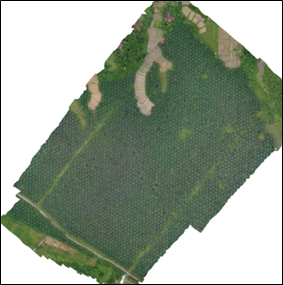
\includegraphics[width=0.5\columnwidth]{bab1/Gambar/Picture1.png}
	\end{center}
	\vspace{-0.2cm}
	%\rule{\columnwidth}{0.1pt}
	\caption{Area Lahan Kelapa Sawit IPB Cargil Jonggol Blok 3 Jarak Tanam 9x9x9}\label{img:bab1-area-lahan-IPB}
\end{figure}
%%%%%%%%%%%%%%%%%%%%%%%%%% GAMBAR %%%%%%%%%%%%%%%%%%%%%%%%%%%%%%

Dalam memenuhi kebutuhan minyak kelapa sawit, selain membutuhkan areal lahan, dibutuhkan pola tanam dan jarak tanam kelapa sawit yang tepat. Pola tanam kelapa sawit yang baik dibutuhkan perhatikan yang lebih karena berkaitan dengan efektifitas penggunaan lahan. Pola tanam segitiga sama sisi merupakan pola tanam yang paling efektif di areal datar, sehingga untuk areal bergelombang atau berbukit perlu dilakukan "viol linning" untuk mempertahankan jumlah populasi per hektarnya dengan tetap memperhatikan tingkat kesuburan tanahnya (GD Morganic, 2018), ilustrasi jarak tanam kelapa sawit seperti pada Gambar \ref{img:bab1-Pola-Tanam-dan-Jarak-Tanam}.

%%%%%%%%%%%%%%%%%%%%%%%%%% GAMBAR %%%%%%%%%%%%%%%%%%%%%%%%%%%%%%
\begin{figure}[H]
	\vspace{-0.1cm}
	%\rule{\columnwidth}{0.1pt}
	\begin{center}
		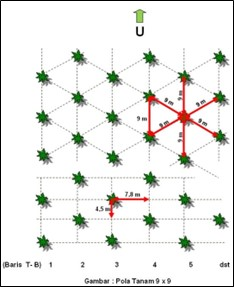
\includegraphics[width=0.5\columnwidth]{bab1/Gambar/Picture2.jpg}
	\end{center}
	\vspace{-0.2cm}
	%\rule{\columnwidth}{0.1pt}
	\caption{Pola Tanam dan Jarak Tanam Kelapa Sawit yang Tepat\\(Sumber: GD Morganic, 2018)}\label{img:bab1-Pola-Tanam-dan-Jarak-Tanam}
\end{figure}
%%%%%%%%%%%%%%%%%%%%%%%%%% GAMBAR %%%%%%%%%%%%%%%%%%%%%%%%%%%%%%

Direktorat Jenderal Perkebunan (Ditjenbun) memetakan memetakan produksi kelapa sawit menurut provinsi dan menunjukkan bahwa provinsi Riau memiliki produksi terbesar 2021 sebesar 8,96 juta ton dengan luas 3,49 juta hektar (Ditjenbun, 2023). Berikut ini Gambar \ref{img:bab1-Peta-10-Besar-Provinsi}. peta kelapa sawit Indonesia berdasarkan Direktorat Jenderal Perkebunan.

%%%%%%%%%%%%%%%%%%%%%%%%%% GAMBAR %%%%%%%%%%%%%%%%%%%%%%%%%%%%%%
\begin{figure}[H]
	\vspace{-0.1cm}
	%\rule{\columnwidth}{0.1pt}
	\begin{center}
		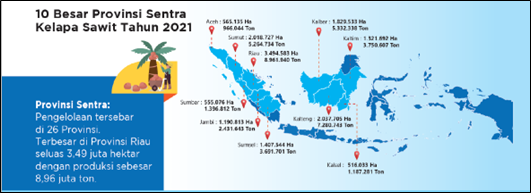
\includegraphics[width=1\columnwidth]{bab1/Gambar/Picture3.png}
	\end{center}
	\vspace{-0.2cm}
	%\rule{\columnwidth}{0.1pt}
	\caption{Peta 10 Besar Provinsi Sentra Kelapa Sawit Tahun 2021\\(Sumber: Ditjenbun, 2023)}\label{img:bab1-Peta-10-Besar-Provinsi}
\end{figure}
%%%%%%%%%%%%%%%%%%%%%%%%%% GAMBAR %%%%%%%%%%%%%%%%%%%%%%%%%%%%%%

Direktorat jenderal perkebunan juga mencatat estimasi luas area dan produksi minyak sawit Indonesia tahun 2023 mencapai 48,24 juta ton dan luas hektar mencapai 15,3 juta ton (Ditjenbun, 2023) seperti pada Gambar  \ref{img:bab1-Estimasi-Luas-Area-Produksi-Minyak}.

%%%%%%%%%%%%%%%%%%%%%%%%%% GAMBAR %%%%%%%%%%%%%%%%%%%%%%%%%%%%%%
\begin{figure}[H]
	\vspace{-0.1cm}
	%\rule{\columnwidth}{0.1pt}
	\begin{center}
		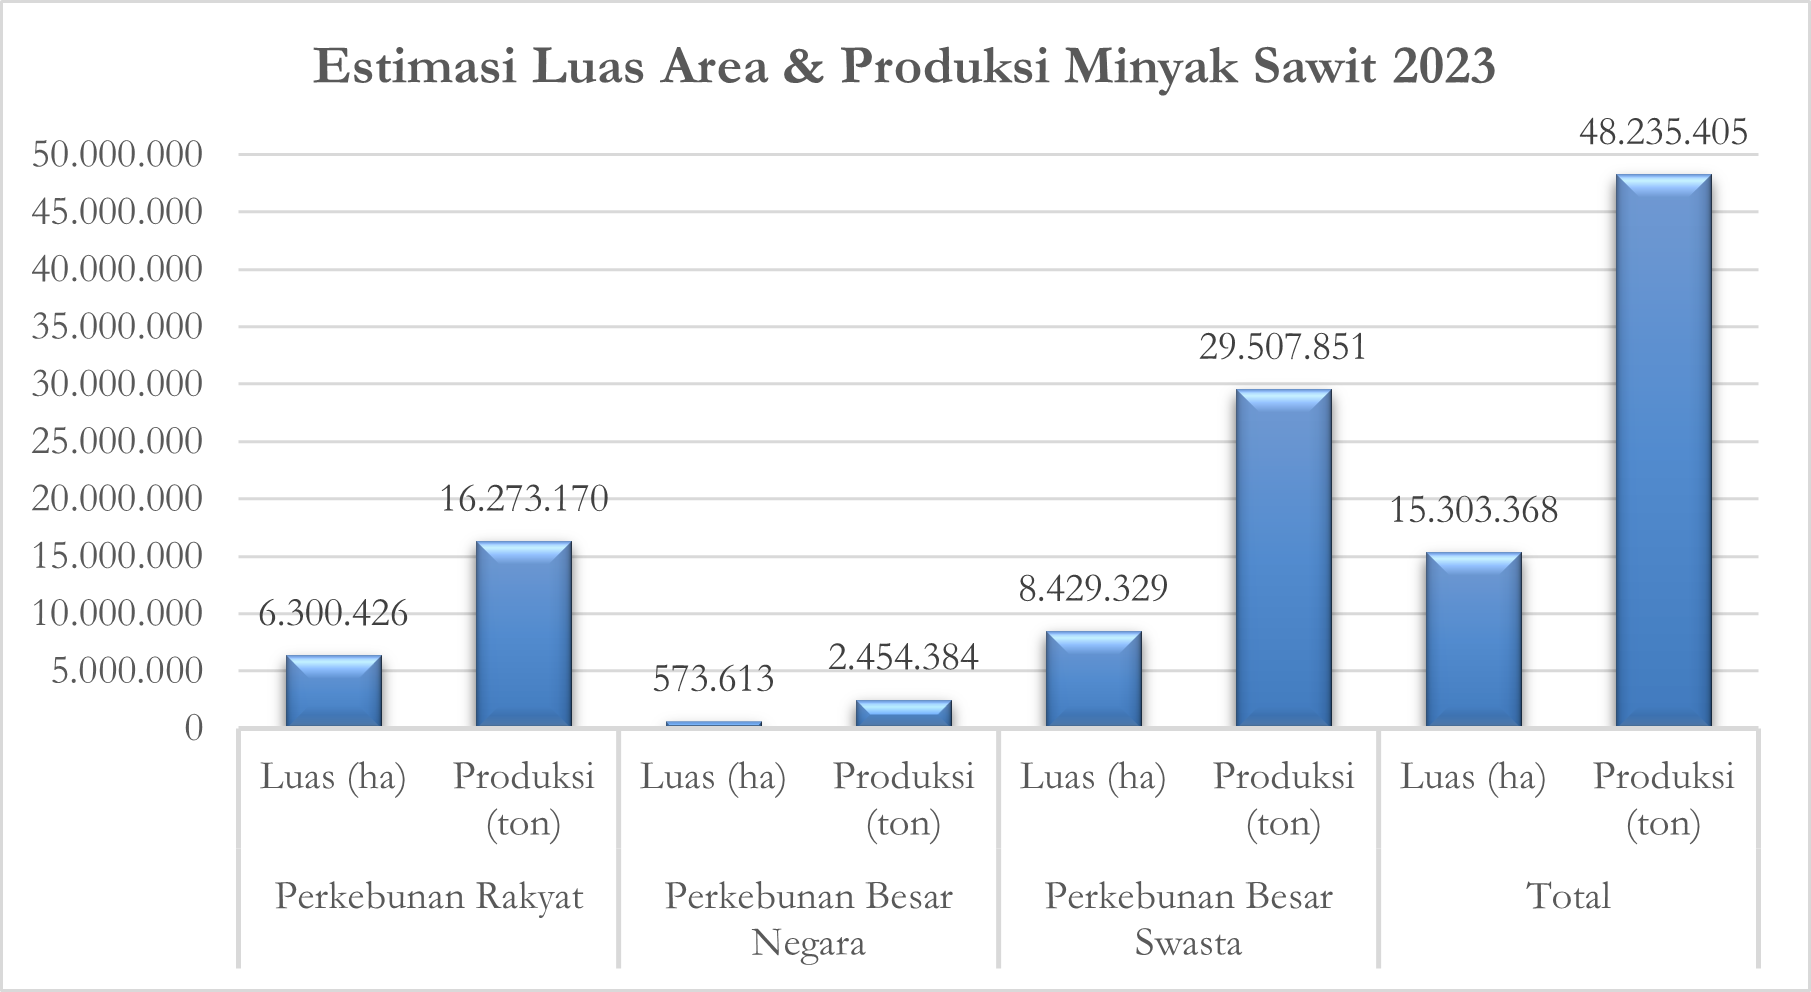
\includegraphics[width=1\columnwidth]{bab1/Gambar/Picture4.png}
	\end{center}
	\vspace{-0.2cm}
	%\rule{\columnwidth}{0.1pt}
	\caption{Estimasi Luas Area dan Produksi Minyak Sawit Indonesia 2023\\Sumber: (Ditjenbun, 2023)}\label{img:bab1-Estimasi-Luas-Area-Produksi-Minyak}
\end{figure}
%%%%%%%%%%%%%%%%%%%%%%%%%% GAMBAR %%%%%%%%%%%%%%%%%%%%%%%%%%%%%%

Gambar \ref{img:bab1-Estimasi-Luas-Area-Produksi-Minyak} menyatakan bahwa perkebunan swasta (PBS) menguasasi sebanyak 61,2\% dengan total produksi 29,5 juta ton, perkebunan rakyat (PR) sebesar 33,7\% dengan total produksi sebanyak 16,2 juta ton, sedangkan perkebunan besar negara (PBN) hanya 5\% dengan total 2,45 juta ton. 

Jumlah estimasi luas area lahan pohon kelapa sawit yang besar juga menjadikan permasalahan bagi pengelolaan perkebunan kelapa sawit. Dari sisi agronomis, bahwa batasan minimum untuk perusahaan perkebunan kelapa sawit yaitu sebesar 6.000 (enam ribu) hektar yang harus dikelola (PPRI, 2021). Luas lahan untuk petani kelapa sawit yang didefinisikan sebagai petani kelapa sawit adalah tingal di pedesaan/sekitar kebun yang dimana kelapa sawit sebagai mat apencaharian utama, dikerjakan dan dikontrol sendiri oleh keluarganya, dan mengalami kesulitan karena bibit yang digunakan disemai sendiri dan tidak bersertifikat, sulit mengakses area karena luas, serta produktivitas rendah menjadi permasalahan utama (SPKS, 2020). Di samping permasalahan luas area ini, lokasi perkebunan sawit juga berada pada remote area, yaitu area atau daerah yang terpencil, jauh dari peradaban (daerah pedalaman atau pelosok hutan) yang dimana karena lokasi perkebunan kelapa sawit yang luas, sehingga sulit dimonitoring tanpa teknologi informasi. Permasalahan yang ada bahwa di perkebunan kelapa sawit yang luas juga terkendala akses infrastruktur, seperti jalan yang belum memadai untuk akses kendaraan, seperti di Kebun Pendidikan dan Penelitian IPB-Cargil akses jalan bergelombang dan masih bebatuan, dan menurut dinas perkebunan provinsi Kalimantan timur bahwa infrastruktur dan aksesibilitas terhubung dengan baik, maka produktivitas dan kegiatan monitoring kawasan perkebunan kelapa sawit akan sangat membantu (Disbun, 2014). Produksi per individu tanaman pohon kelapa sawit berkontribusi besar terhadap produktivitas karena setiap pohon kelapa sawit akan menghasilkan buah kelapa sawit yang dapat diproduksi dan dipanen hasilnya untuk masyarakat, sehingga data pohon kelapa sawit sangat penting untuk dilakukan. Selain itu, salah satu upaya yang dilakukan dalam perkebunan kelapa sawit adalah masalah pemupukan. Adanya peningkatan produksi melalui intensifikasi dengan pemberian pupuk yang presisi, secara cepat, dan akurat, serta up-to-date pada suatu luasan lahan.  Upaya yang dapat dilakukan adalah dengan meningkatkan produktivitas melalui peningkatan efektivitas dan efisiensi penggunaan pupuk. Efektivitas dan efisiensi pemberian pupuk sangat penting dilakukan karena biaya pemupukan tanaman kelapa sawit sangat besar yaitu 50\%-70\% dari biaya pemeliharaan dan 25\% dari seluruh biaya produksi (Fairhurst et al., 2006). Penambahan unsur hara dapat meningkatkan pertumbuhan tanaman, produksi tanaman, dan kualitas produk yang dihasilkan, seperti buah kelapa sawit (S. Parman, 2007).	

Buah kelapa sawit yang dapat dihasilkan di Indonesia cukup besar dan harus diproduksi atau dipanen dengan baik, agar hasil dari buah kelapa sawit yang mayoritas menjadi minyak menghasilkan minyak yang berkualitas. Hal ini berkenaan dengan standar mutu kematangan buah kelapa sawit yang dikenal dengan standar kematangan panen. Buah sawit bergerombol dalam tandan yang muncul dari tiap pelapah. Minyak dihasilkan oleh buah. Kandungan minyak bertambah sesuai dengan tingkat kematangan buah. Penghitungan pohon kelapa sawit yang menghasilkan minyak dapat dilakukan secara manual di lapangan, tetapi ini menghabiskan waktu, membutuhkan pekerja yang tidak sedikit, dan mahal (N. A Mubin, et al, 2019). Disamping itu, Manajer perkebunan kelapa sawit biasanya mengukur kepadatan kelapa sawit secara manual setiap tahun. Data penting ini dapat digunakan untuk memperkirakan produktivitas kelapa sawit, jumlah pupuk yang dibutuhkan, biaya penyiangan berkala, dan jumlah pekerja yang dibutuhkan, dan terkait dengan kegiatan lain (J. W. Kiama, 2014).

Oleh karena itu, dibutuhkan suatu metode atau teknologi untuk membantu mengklasifikasikan atau mendeteksi jumlah dan estimasi usia pohon kelapa sawit untuk dapat diketahui tingkat kematangan buah kelapa sawit, maka dapat diproduksi (dipanen) dengan baik, sehingga produksi yang dihasilkan dapat mencapai optimum. Berikut ini penelitian-penelitian yang telah dilakukan penelitian sebelumnya.

Klasifikasi berbasis piksel sering digunakan untuk mengklasifikasikan kelas fitur dari gambar. Metode Object-Based Image Analysis (OBIA) telah berevolusi untuk menganalisis gambar resolusi tinggi dengan cepat (T. Blaschke, 2010), dengan semakin tersedianya resolusi tinggi dan citra skala besar, maka dihasilkan cara baru untuk memulai penelitian tentang interpretasi foto pohon berbasis komputer (P. Gong et al, 1999). OBIA dikembangkan oleh Hay dan Castilla merupakan disiplin ilmu spasial yang berfokus pada pengelompokkan citra penginderaan jauh ke makna objek penuh melalui pemanfaatan spasial (G. J. Hay et al, 2008). Gagasan menganalisis gambar dalam ruang objek daripada ruang pixel dikembangkan karena kekurangan metode berbasis pixel, terutama pada gambar resolusi tinggi. Selain itu, ruang objek telah diperkuat dalam kapasitas komputasi dan ketersediaan untuk analisis gambar resolusi tinggi seperti IKONOS, GeoEye, dan WorldView (T. Blaschke, 2010).

Jusoff dan Pathan menggunakan airborne hyperspectral sensing linear analis campuran spectral, bersama dengan campuran ke konventer murni dan norma Euclidean teknik untuk memetakan masing-masing pohon kelapa sawit (K. Jusoff, 2009). Korom et all tahun 2014 mengelompokkan bentuk kanopi atau mahkota kelapa sawit menggunakan citra WorldView-2 berdasarkan segmentasi watershed dan mencapai akurasi sekitar 77\% \citep{Korom2014-ci}.

Wong-in et al. tahun 2015 telah mencapai akurasi 90\% menggunakan gambar udara dengan beberapa langkah, seperti menghapus komponen non-pohon dari gambar, membedakan munyak sawit dari komponen lain menggunakan filter low-pass dan korelasi silang dinormalisasi, mengidentifikasi pohon kelapa sawit secara individu dan menghitung jumlah pohon kelapa sawit (Wong-in et al, 2015).

H. Santoso et al. pada tahun 2016 membangun dan mengembangkan metode yang mudah digunakan pengguna yang akan memungkinkan manajer kelapa sawit untuk menghitung minyak pohon kelapa sawit menggunakan teknik penginderaan jauh. Pohon kelapa sawit dianalisis dalam penilitian ini dengan melihat usia dan kepadatan yang berbeda. Penelitian ini menggunakan Citra QuickBird yang diaplikasikan dengan enam metode pansharpening. Hitam dan citra putih dari komposit warna palsu citra pansharpening diproses dalam tiga cara: (1) deteksi pohon kelapa sawit, (2) penggambaran area kelapa sawit, (3) penghitungan pohon kelapa sawit dan penilaian akurasi. Penelitian ini menggunakan ENVI 5.2, ERDAS Imagine 2015, dan ArcGIS 10.2.2. Hasil penelitian ini meningkat pada akurasi dari beberapa studi penelitian sebelumnya yang memiliki akurasi 90-95\%. Hasil dalam penelitian ini menunjukkan (1) gabungan resolusi intensitas huesaturation (HIS) cocok untuk kelapa sawit berusia 16 tahun, pohon dan memiliki kepadatan agak tinggi dengan akurasi 100\%, (2) untuk kelapa sawit berusia 21 tahun dan memiliki kepadatan rendah didapatkan hasil dengan akurasi 99,5\%, (3) resolusi subtraktif penggabungan ini cocok untuk pohon kelapa sawit berusia 15-18 tahun dan memiliki kerapatan yang agak tinggi dengan akurasi 99,8\%, (4) penajaman spectral PC dengan akurasi 99,3\% cocok untuk pohon kelapa sawit berusia 10 tahun dan memiliki kepadatan rendah, dan (5) untuk semua kondisi objek studi, warna dinormalisasi (Brovey) dan penggabungan resolusi wavelet adalah dua metode pansharpening yang cocok untuk ekstraksi dan kelapa sawit dengan penghitungan masing-masing dengan akurasi 98,9\% dan 98,4\% (H. Santoso et al, 2016).

H. M. Rizeei et al. tahun 2018 meneliti bahwa pemantauan karakteristik kelapa sawit di area perkebunan sangat berharga bagi petani dan stakeholders untuk memaksimalkan produktivitas. Penelitian ini mengusulkan metode baru untuk estimasi dan penghitungan usia kelapa sawit. Algoritma Support Vector Machine (SVM) dari analisis gambar berbasis objek (OBIA) diterapkan untuk penghitungan kelapa sawit. Analisis sensitivitas dilakukan pada empat jenis kernel SVM (Sigmoid (SIG), Linear (LN), fungsi basis radial (RBF), dan polynomial (PL)) dengan parameter terkait (Nilai ambang batas, Gamma ($\gamma$) dan faktor Penalti (c )) untuk mendapatkan pendekatan klasifikasi OBIA optimal untuk setiap blok perkebunan. Citra dengan resolusi sangat tinggi dari Worldview-3 (WV-3) digunakan untuk deteksi kelapa sawit. Hasil deteksi kelapa sawit memiliki akurasi keseluruhan 98,27\%, 99,48\%, 99,28\%, 99,49\%, dan 97,49\% untuk blok A, B, C, D, dan E (H. M. Rizeei, 2018).

W Li et al tahun 2018 meneliti deteksi pohon kelapa sawit dalam skala besar dari gambar satelit beresolusi tinggi (QuickBird) menggunakan Two-Stage Convolutional \textit{Neural Networks} (TS-CNN). TS-CNN terdiri dari satu CNN untuk klasifikasi tutupan lahan dan satu CNN untuk klasifikasi objek. Kedua CNN dilatih dan dioptimalkan secara independen berdasarkan pada 20.000 sampel yang dikumpulkan melalui interpretasi manusia. Skala area pohon kelapa sawit sebesar 55 km2. Penelitian ini mengusulkan alur kerja yang efektif yang terdiri dari metode partisi yang tumpeng tindih untuk divisi gambar skala besar, metode \textit{multi-scale sliding window} untuk memprediksi koordinat kelapa sawit, dan metode filter jarak untuk pasca-pemrosesan. Pendekatan yang diusulkan mencapai skor F1 rata-rata yang jauh lebih tinggi yaitu 94,99\% di wilayah studi dibandingkan dengan metode deteksi kelapa sawit yang ada masing-masing sebesar (87,95\%, 81,80\%, 80,61\%, dan 78,35\% untuk CNN satu-tahap, \textit{Support Vector Machine} (SVM), \textit{Random Forest} (RF), dan \textit{Artificial Neural Network} (JST)), dan jauh lebih sedikit kebingungan dengan vegetasi dan bangunan lain di seluruh hasil deteksi gambar (W. Li et al, 2019).

N. A. Mubin et al. tahun 2019 telah meneliti bahwa deteksi dan penghitungan kelapa sawit penting dalam pengelolaan perkebunan kelapa sawit. Dalam penelitian ini, digunakan pendekatan pembelajaran mendalam untuk memprediksi dan menghitung kelapa sawit dalam citra satelit. Deteksi kelapa sawit sebelumnya secara umum berfokus pada mendeteksi kelapa sawit yang tidak memiliki tumpeng tindih mahkota. Selain itu, terdapat kurangnya penelitian yang membangun sistem deteksi terpisah untuk kelapa sawit muda dan dewasa, memanfaatkan pendekatan pembelajaran mendalam untuk mendeteksi kelapa sawit dan menggabungan sistem informasi geografis (SIG) dengan pendekatan pembelajaran mendalam. Penelitian ini mencoba untuk mengisi kesenjangan ini dengan memanfaatkan dua jaringan saraf convolution (CNN) yang berbeda untuk mendeteksi kelapa sawit muda dan matang secara terpisah dan menggunakan GIS selama pemrosesan data dan proses penyimpanan hasil. Arsitektur awal yang dikembangkan didasarkan pada CNN yang disebut LeNet. Proses pelatihan mengurangi kerugian dengan menggunakan algoritma gradient adaptif dengan batch mini ukuran 20 untuk semua set pelatihan yang digunakan. Kemudian, mengekspor hasil prediksi ke perangkat lunak GIS dan membuat peta prediksi kelapa sawit dewasa dan muda. Berdasarkan metode yang diusulkan, akurasi keseluruhan untuk kelapa sawit muda dan matang masing-masing adalah 95,11\% dan 92,96\%. Secara keseluruhan, pengklasifikasi bekerja dengan baik pada dataset yang sebelumnya tidak terlihat, dan mampu secara akurat mendeteksi kelapa sawit dari latar belakang, termasuk bayangan tanaman lainnya (N. A. Mubin, 2019). 

\section{Batasan Penelitian}
\label{sec:2-BatasanMasalah}
\hspace{1,2cm}Ruang lingkup yang menjadi penelitian adalah:
\begin{enumerate}
	\item Dataset citra sebagai dataset primer berjumlah 69 citra dari Kebun Pendidikan dan Penelitian Kelapa Sawit IPB-Cargil, Jonggol, Jawa Barat dan 205 citra dari Universitas Gunadarma, PPU Campus, Kalimantan Timur yang ditanami pohon kelapa sawit.
	\item Dataset sekunder digunakan melalui akses roboflow secara free sebanyak 1795 citra dataset sekunder yang sudah memiliki label atau anotasi kelas 'oil palm'.
	\item Pengujian penerapan sistem menghitung dan mendeteksi pohon kelapa sawit dilakukan pada lahan pohon kelapa sawit tanah mineral Kebun Pendidikan dan Penelitian Kelapa Sawit IPB-Cargil, Jonggol Jawa Barat.
\end{enumerate}


\section{Rumusan Masalah}
\label{sec:3-Rumusanmasalah}
\hspace{1,2cm}Adapun rumusan masalah dalam penelitian ini secara umum bahwa pengelolaan perkebunan kelapa sawit memiliki permasalahan yang utama, diantaranya luas area pengelolaan kebun kelapa sawit dalam skala besar (perusahaan perkebunan kelapa sawit memiliki luas minimum sebesar 6.000 (enam ribu) hektar dan petani 4 hektar yang harus dikelola). Perkebunan berada di \textit{remote area}, area yang terpencil, daerah pedalaman atau pelosok hutan, yang sulit untuk dilakukan monitoring, dan akses infrastruktur terutama jalan yang terbatas dan sulit. Permasalahan yang dihadapi juga berupa pemupukan presisi yang mengalami kesulitan untuk mendapatkan secara akurat, dan cepat, serta \textit{up-to-date} jumlah tegakkan pohon kelapa sawit pada suatu luasan lahan tertentu, sementara praktik yang ada adalah menggunakan perhitungan manual dan normatif berbasis jarak tanam pohon kelapa sawit. Hal ini menyebabkan pentingnya data jumlah pohon kelapa sawit sangat penting dibutuhkan karena produksi per individu tanaman berkontribusi besar terhadap produktivitas dengan penyelesaian teknologi informasi. Berdasarkan permasalahan tersebut, maka rumusan masalah secara khusus:  
\begin{enumerate}
	\item Bagaimana membuat pengembangan metode \textit{object-based image analysis} (OBIA) untuk membuat dataset secara otomatis dengan memberikan anotasi atau label suatu kelas pada data citra?
	\item Bagaimana mendapatkan model CNN yang baik dari algoritma YOLOv5, YOLOv6, dan YOLOv7 untuk mendeteksi dan menghitung pohon kelapa sawit pada suatu area tertentu?
	\item Bagaimana mengembangkan sistem berbasis web dengan menerapkan model CNN dari algoritma YOLO agar dapat mendeteksi, menghitung, dan mendapatkan letak koordinat latitude-longitude setiap pohon kelapa sawit dari citra satelit agar dapat dilakukan pemantauan, pengelolaan, dan estimasi produktivitas secara otomatis?
\end{enumerate}

\section{Tujuan Penelitian}
\label{sec:4-BatasanMasalah}
\hspace{1,2cm}Adapun tujuan dari penelitian ini secara umum adalah menghasilkan purwarupa sistem berbasis web dengan menerapkan model OBIA dan \textit{Deep Learning} (DL) untuk mendeteksi, menghitung jumlah pohon dalam suatu luasan tertentu dan mendapatkan nilai koordinat latitude-longitude setiap pohon kelapa sawit dari citra satelit. Tujuan penelitian secara khusus sebagai berikut: 
\begin{enumerate}
	\item Menghasilkan metode object-based image analysis (OBIA) untuk membuat dataset secara otomatis dengan memberikan anotasi atau label suatu kelas, kelas 'oil palm' pada data citra.
	\item Menghasilkan model CNN dari algoritma YOLOv5, YOLOv6, dan YOLOv7 yang dapat mendeteksi dan menghitung pohon kelapa sawit pada suatu area tertentu.
	\item Menghasilkan purwarupa perangkat lunak aplikasi dengan model convolutional neural network dari algoritma YOLO yang terintegrasi dengan citra satelit dengan menggunakan Google Maps API yang dapat mendeteksi, menghitung, dan mendapatkan letak koordinat latitude-longitude setiap pohon kelapa sawit pada suatu area tertentu.
\end{enumerate}

\section{Kontribusi Hasil Penelitian}
\label{sec:5-Kontribusi-Hasil-Penelitian}
\hspace{1,2cm}Kontribusi penting dari penelitian yang dilakukan dalam penelitian ini adalah:
\begin{enumerate}
	\item Dari sisi keilmuan, berupa pengembangan metode \textit{object-based image analysis} (OBIA) untuk membuat dataset secara otomatis dengan memberikan anotasi atau label suatu kelas pada data citra dengan menggunakan algoritma \textit{template matching} dan BIRCH.
	\item Dari sisi teknologi, penelitian ini menghasilkan dataset primer dengan kelas pohon kelapa sawit (\textit{oil palm}) dan purwarupa perangkat lunak aplikasi dengan model \textit{convolutional neural network} dari algoritma YOLO yang terintegrasi dengan citra satelit dengan menggunakan Google Maps API yang dapat mendeteksi, menghitung, dan mendapatkan letak koordinat latitude-longitude setiap pohon kelapa sawit yang berhasil dideteksi.
	3.	Dari sisi pemanfaatan, menawarkan suatu cara alternatif untuk proses persiapan data citra untuk mendapatkan dataset dengan proses anotasi yang lebih cepat, serta bagi \textit{stakeholder} dapat memantau, mengelola, dan melakukan estimasi produktivitas secara otomatis pohon kelapa sawit pada suatu area tertentu dengan penerapan teknologi informasi.
	
\end{enumerate}

%%%%%%%%%%%%%%%%%%%%%%%%%%% GAMBAR %%%%%%%%%%%%%%%%%%%%%%%%%%%%%%
%\begin{figure}[!h]
%  \vspace{-0.1cm}
%%\rule{\columnwidth}{0.1pt}
%\begin{center}
%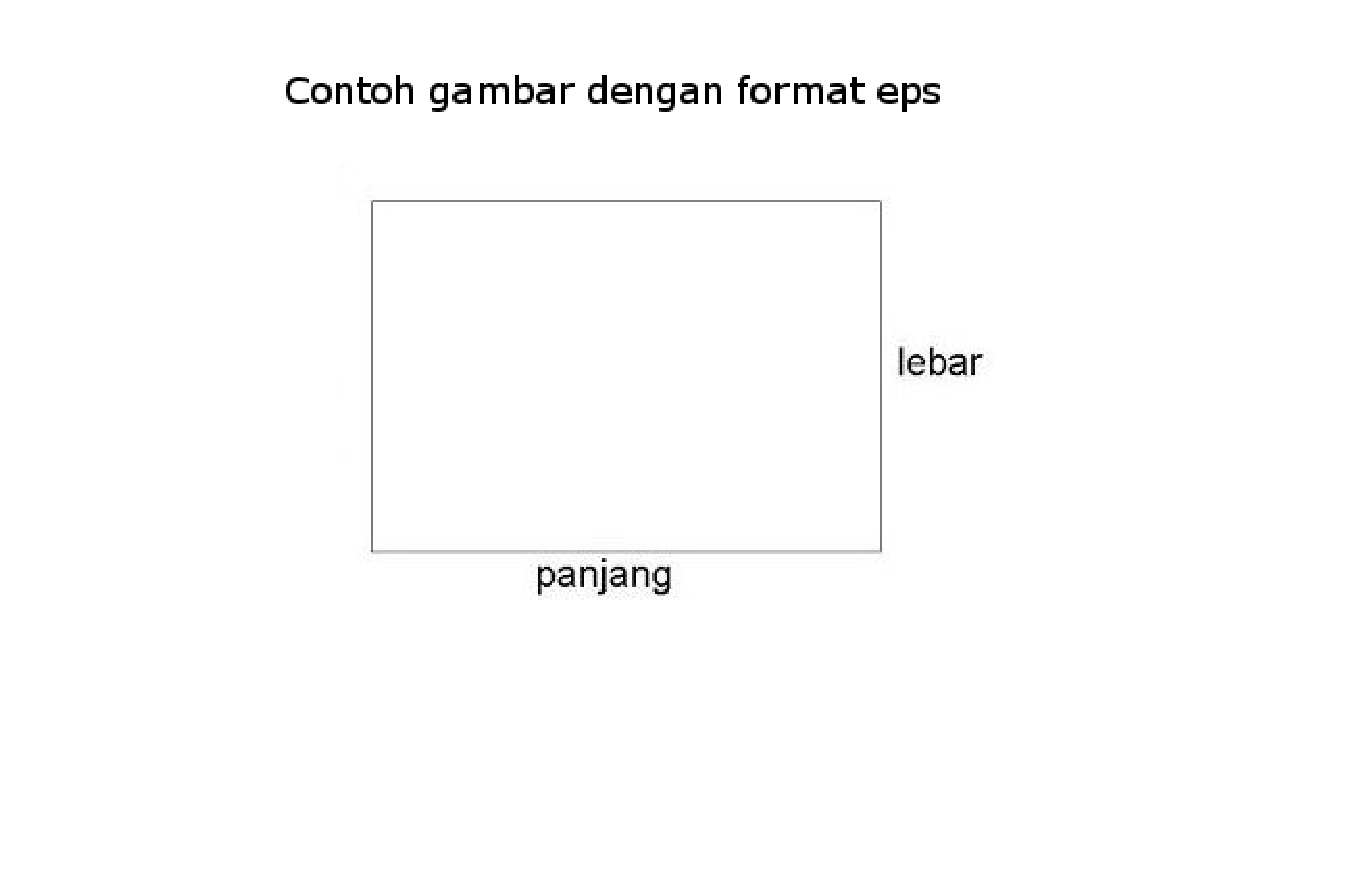
\includegraphics[width=0.8\columnwidth]{bab1/Gambar/gambar1-1.eps}
%\end{center}
%\vspace{-0.2cm}
%%\rule{\columnwidth}{0.1pt}
%\caption{Perbedaan Alur Desain FPGA dan Desain ASIC}\label{gambar1}
%\end{figure}
%%%%%%%%%%%%%%%%%%%%%%%%%%% GAMBAR %%%%%%%%%%%%%%%%%%%%%%%%%%%%%%

